\documentclass[12pt]{book}
\usepackage[a4paper, portrait, inner=2cm, outer=3cm, top=2.5cm, bottom=2.5cm]{geometry}

\usepackage{tikz}
\usepackage{lipsum}
\usepackage{graphics}
\usepackage{pdfpages}
\usepackage{fancyhdr}
\usepackage{graphicx}
\usepackage{multicol}
\usepackage{multirow}
\usepackage{tabularx}

% Removes boxes from links
\usepackage[
    colorlinks=true,
    linkcolor=black,
    anchorcolor=black,
    citecolor=black,
    filecolor=black,
    menucolor=black,
    runcolor=black,
    urlcolor=black
]{hyperref}

% Disable default indentation an add paragraph spacing
\usepackage[parfill]{parskip}

\graphicspath{{images/} {../images}}

\input{definitions/000-plain-page-header-fix}
\input{definitions/001-center-page}

\usepackage[cmintegrals,cmbraces]{newtxmath}
\usepackage{ebgaramond-maths}
\usepackage[T1]{fontenc}

\usepackage{subfiles}

\title{PDen OS Book - C - Zero To Hero}
\author{Tyler Dence, et. al.}
\date{April 2021}

\begin{document}

% Start book 
\frontmatter
    % Set page number to zero
    % This makes the cover take page zero,
    % which puts the first content at page 1.
    \setcounter{page}{0}
    
    % Cover
    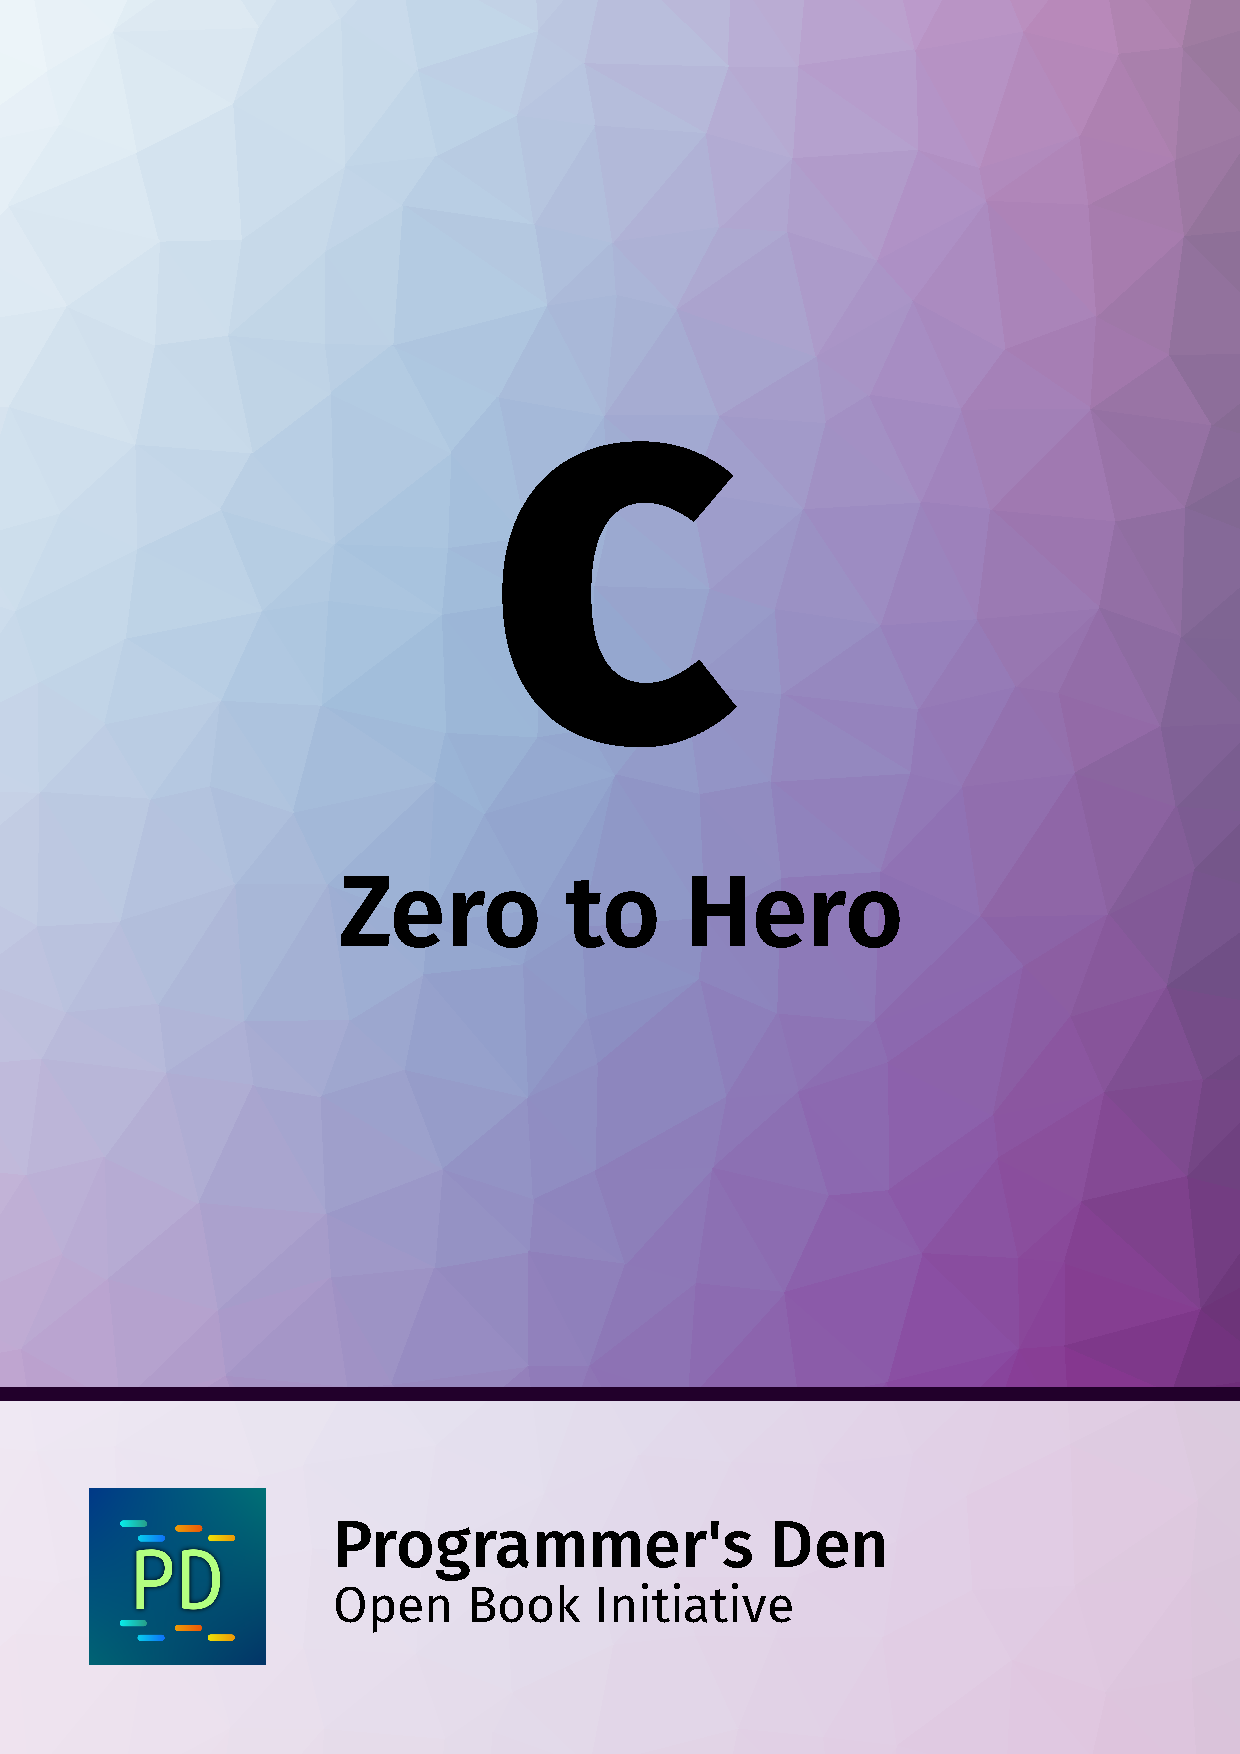
\includepdf[pages=-]{images/cover}
    
    % Front sections 
    \subfile{chapters/0.0-foreword}
    \subfile{chapters/0.1-copyright}
    
    % Create table of contents
    \tableofcontents
    
    % Fix header bug where "CONTENTS"
    % shows up in header of blank page
    \clearpage
    \markboth{}{}

% Chapters
\mainmatter
    \subfile{chapters/1.0-introduction}

\end{document}
